% !TEX root = ../../math6370.tex

\section{Dedekind Zeta Function}
\subsection{Calculating $\Cl_K$ and $\O_K^\times$ \label{sec:count}}

Since this section will pull together much of the theory and notation developed thus far, we begin by reminding the reader of the notation as well as establishing two new notational conveniences: $\omega_K$, $h_K$. \\

Let $K/\Q$ be a number field. Then define\dots

\begin{itemize}
\item $n=[K \colon \Q]$
\item $r$, the number of real embeddings $\sigma: K \hra \R \subseteq \C$
\item $s$,  the number of complex conjugate pairs of embeddings, $\sigma: K \hra \C$, $\sigma(K) \not\subseteq \R$
\item $\disc K \in \Z$, the discriminant of $K$
\item $\O_K^\times$, the group of units of $\O_K$ (which will be of rank $r+s-1$)
\item $\phi: \O_K^\times \to V:=\{x \in \R^{r+s} \colon \sum_i x_i=0\}$ given by $\alpha \mapsto (e_i\log|\sigma_i(\alpha)|)_i$, where $e_i=1$ for $1 \leq i \leq r$ and $e_i=2$ for $r+1 \leq i \leq r+s$
\item $\reg_K:=\frac{1}{\sqrt{r+s}} \covol(\phi(\O_K^\times))>0$, the regulator of $K$
\item $\omega_K:= \#\mu_K \in \Z^+$, the group of roots of unity in $K$
\item $h_K:=\#\Cl_K \in \Z^+$, where $\Cl_K$ is the class group of $K$ (which will be a finite abelian group)
\end{itemize}

Up to this point, we have computed some elementary examples of $\Cl_K$ and $\O_K^\times$. But we have yet to give an effective algorithm for computing these in general. Assuming one can numerically compute $h_K \reg_K$, we give an ``effective'' algorithm to calculate both $\Cl_K$ and $\O_K^\times$ (modulo some terms `many', `guess', and `enough', which we shall leave ill defined for our purpose). One can then use $\Cl_K$ and $\O_K^\times$ to compute $h_K$ and $\reg_K$ exactly. However, we shall describe in later sections a method of computing $h_K \cdot \reg_K$ so that this algorithm will not be circular. Strangely enough, it is simpler to compute $h_K \cdot \reg_K$ than either $h_K$ or $\reg_K$ individually. In any case, the algorithm is as follows:

\begin{enumerate}[1.]
\item Compute primes $\p_1,\ldots,\p_m$ with $N(\p_i) \leq M_K$, where $M_K$ is the Minkowski constant for $K$. 

\item Find `many' factorizations $\alpha_i \O_K= \p_1^{a_{i,1}} \cdots \p_m^{a_{i,m}}$ with $1 \leq i \leq M$ (the number of factorizations found) and $\alpha_i \in K$. 

\item Define a `guess' for $O_K$: $C:= \Z^m/\langle \{(a_{i,1},\ldots,a_{i,m}) \colon 1 \leq i \leq M\} \rangle$ (being sure to find `enough' relations so that $C$ is finite). Now $C \twoheadrightarrow \Cl_K$ under the map $e_i \mapsto [\p_i]$, where $e_i$ is the $i$th standard basis vector. Note then $(a_{i,1},\ldots,a_{i,m}) \mapsto [\p_1]^{a_{i,1}} \cdots [\p_m]^{a_{i,m}}=[\alpha \O_K]=1$. The map is surjective since $\p_1,\ldots,\p_m$ generate $\Cl_K$. This map will be an isomorphism if we have found `enough factorizations to find all the relations in $\Cl_K$.

\item Take $(b_1,\ldots,b_M) \in \Z^M$ such that $\sum_{i=1}^M a_{i,j} b_i=0$ for all $1 \leq j \leq M$. This says that $\prod_{i=1}^M (\alpha_i \O_K)^{b_i}=\prod_{i=1}^M \alpha_i^{b_i} \O_K= \O_K$ (collecting the exponent of $[\p_i]$, one finds the total is zero). Then $\prod_{i=1}^M \alpha_i^{b_i} \in \O_K^\times$. Let $U \subseteq \O_K^\times$ be the group generated by these units (being sure one has found enough so that $U$ has rank $r+s-1$) along with $\mu_K$. We will have $U=\O_K^\times$ for `enough' factorizations.

\item Now $\frac{\#C}{\#\Cl_K}$ is a positive integer. We have $\frac{\covol(\phi(U))}{\covol(\phi(\O_K^\times))}=[\phi(\O_K^\times) \colon \phi(U)]=[\O_K^\times \colon U]$ (as both contain the roots of unity). But
	\[
	\underbrace{\dfrac{\#C}{\sqrt{r+s}} \;\covol(\phi(U))}_{\text{Computable}} = \underbrace{\dfrac{\#C}{\#\Cl_K} \cdot [\O_K^\times \colon U]}_{\text{``}\in\, \Z^+\text{''}} \cdot \underbrace{h_K \reg_K}_{\text{Known}}.
	\]
By assumption, $h_K \reg_K$ is known. The number $\frac{\#C}{\sqrt{r+s}} \;\covol(\phi(U))$ is effectively computable. Finally, $\dfrac{\#C}{\#\Cl_K} \cdot [\O_K^\times \colon U] \in \Z^+$ theoretically. However in practice, we will know this only as an approximation in $\R^+$. Once this number is `numerically 1', $\#C=\#\Cl_K$ and $[\O_K^\times \colon U]=1$. Then $C \twoheadrightarrow \Cl_K$ is a surjective map between finite groups of the same size so that it is an isomorphism. We have also clearly calculated the unit group. 
\end{enumerate}





\subsection{Counting Ideals}

While the above algorithm was useful, it rested on the assumption that one could calculate $h_K \reg_K$. It remains to show that one can effectively compute $h_K \reg_K$. We calculate this by counting ideals.

\begin{dfn}
Let $x \in \R$. Define
	\[
	\A(x):= \#\{ 0 \neq I \subseteq \O_K \colon N(I) \leq \}.
	\]
\end{dfn}

For $x\leq 0$, $\A(x)=0$ and $\A(x)$ is finite for $x \in \R$ as there are only finitely many ideals of a given norm. A natural question to ask is how does $\A(x)$ grow with $x$? This leads to the class number.

\begin{thm}[Analytic Class Number]
There exists a constant $\kappa$, called the class number, such that $\A(x) \sim \kappa x$ as $x \to \infty$. Moreover,
	\[
	\kappa= \dfrac{2^r (2\pi)^s h_K \reg_K}{\omega_K |\disc K|^{1/2}}.
	\]
\end{thm}

\noindent \emph{Proof (Sketch). } Fix $C \in \Cl_K$ and define
	\[
	\A(x,C):= \#\left\{ I \subseteq \O_K \colon N(I) \leq x, [I]=C \right\}.
	\]
Note that $\A(x)=\sum_{C \in \Cl_K} \A(x,C)$. It suffices to prove
	\[
	\A(x,C) \sim \dfrac{2^r (2\pi)^s \reg_K}{\omega_K |\disc K|^{1/2}}
	\]
since there are $h_K$ such $\A(x,C)$ in total. We shall prove the theorem in the case where $K/\Q$ is quadratic. The general case works the same but merely involves (extreme) `bookkeeping'.

Fix an ideal $J$ with $[J]=C^{-1}$. For $I$ with $[I]=C$ and $N(I) \leq x$, we have $IJ=(\alpha)$ for some $\alpha \in J$ and
	\[
	|\Nm{K/\Q}(\alpha)|= N(\alpha \O_K)= N(IJ)= N(I)N(J) \leq xN(J).
	\]
Conversely, choose $0 \neq \alpha \in J$ with $|\Nm{K/\Q}(\alpha)| \leq x N(J)$. Then $(\alpha) \subseteq J$, which implies $I:=(\alpha)J^{-1}$ is an ideal with
	\[
	N(I)= \dfrac{|\Nm{K/\Q}(\alpha)|}{N(J)} \leq \dfrac{xN(J)}{N(J)}= x.
	\]
Therefore, this shows
	\[
	\A(x,C)= \# \left\{ (\alpha) \colon 0 \neq \alpha \in J, \Nm{K/\Q}(\alpha) \leq x N(J). \right\}.
	\]
It remains to count $\alpha \in J$, which leads to lattices. [Note, we count up to units since if $u$ is a unit, $(u\alpha)=(\alpha)$.] \\

\noindent \emph{Case 1, $K/\Q$ imaginary quadratic}: We have $\O_K^\times=\mu_K$ and $\A(x,C)=\#(J \cap D_x)$, where 
	\[
	D_x= \left\{ z \in \C \colon 0 \leq \text{Arg}(z)< \dfrac{2\pi}{\omega_K}, z\overline{z} \leq x N(J) \right\}. 
	\]
The set $D_x$ simply induces rotation on nonzero elements. Note that any principal ideal of $\O_K$ has a unique, nonzero generator $\alpha$ with $0\leq \text{Arg}(\alpha) < 2\pi/\omega_K$ and norm $\Nm{K/\Q}(\alpha)=\alpha\overline{\alpha}>0$. 

	\begin{figure}[H]
	\centering
	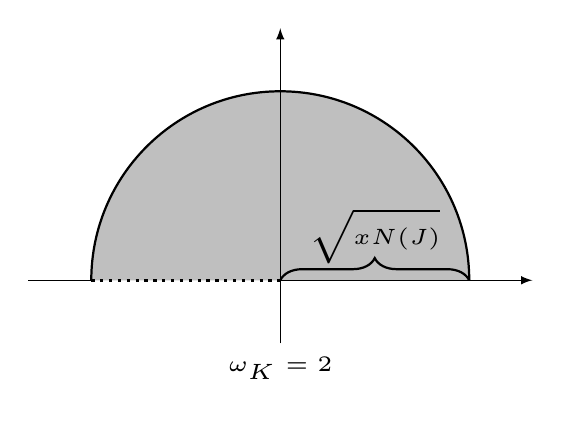
\begin{tikzpicture}[thick,scale=1.6, every node/.style={transform shape}]
		\node at (0,-0.7) {\tiny{$\omega_K=2$}};
		\draw[thick,fill=lightgray] (1.5,0) arc(0:180:1.5);
		\draw[dotted,very thick] (-1.5,0) -- (0,0);
		\draw [decorate,decoration={brace,amplitude=8pt},xshift=0pt,yshift=0pt]
(0.0,0) -- (1.5,0) node [black,midway,xshift=0cm,yshift=0.35cm] {\tiny $\sqrt{xN(J)}$};
		
    		\coordinate (XAxisMin) at (-2,0);
    		\coordinate (XAxisMax) at (2,0);
    		\coordinate (YAxisMin) at (0,-0.5);
    		\coordinate (YAxisMax) at (0,2);
		\draw[thin] (XAxisMin) -- (-1.5,0);
    		\draw [thin,-latex] (0,0) -- (XAxisMax);% Draw x axis
    		\draw [thin,-latex] (YAxisMin) -- (YAxisMax);% Draw y axis	
	\end{tikzpicture} 
	 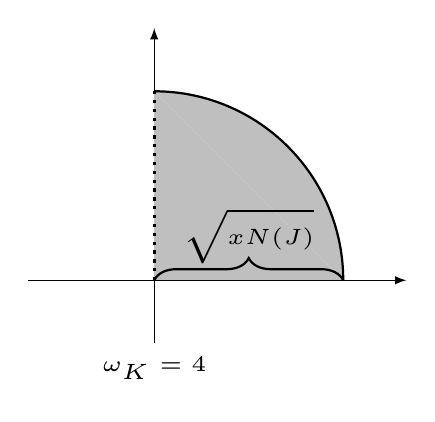
\begin{tikzpicture}[thick,scale=1.6, every node/.style={transform shape}]
		\node at (0,-0.7) {\tiny{$\omega_K=4$}};
		\draw[thick,fill=lightgray] (1.5,0) arc(0:90:1.5);
		\fill [lightgray,domain=0:1.5, variable=\x]
		(0,0)
		-- plot ({\x},{1.5-\x})
		-- (1.5,0)
		-- cycle;
		\draw [decorate,decoration={brace,amplitude=8pt},xshift=0pt,yshift=0pt]
(0.0,0) -- (1.5,0) node [black,midway,xshift=0cm,yshift=0.35cm] {\tiny $\sqrt{xN(J)}$};
		
    		\coordinate (XAxisMin) at (-1,0);
    		\coordinate (XAxisMax) at (2,0);
    		\coordinate (YAxisMin) at (0,-0.5);
    		\coordinate (YAxisMax) at (0,2);
		\draw[thin,-latex] (0,1.5) -- (YAxisMax);
    		\draw [thin,-latex] (XAxisMin) -- (XAxisMax);% Draw x axis
    		\draw [dotted,very thick] (0,0) -- (0,1.5);% Draw y axis
		\draw[thin] (0,-0.5) -- (0,0); 
	\end{tikzpicture}  
	\caption{The region $D_x$ for $\omega_K=2$ (left) and $\omega_K=4$ (right). \label{fig:wkregions}}
	\end{figure}
	
Then as $x$ tends to infinity,
	\[
	\A(x,C) \sim \dfrac{\text{Area}(D_x)}{\covol J} = \dfrac{\dfrac{\pi \sqrt{x N(J)}^2}{\omega_K}}{|\disc K|^{1/2} \cdot N(J)/2}= \dfrac{2\pi}{\omega_K |\disc K|^{1/2}} \; x
	\]

\noindent \emph{Case 2, $K/\Q$ real quadratic}: Let $K \subseteq \R$ be a real quadratic field and let $\tau: K \hra \R$ be the non-identity embedding. By Dirichlet's Unit Theorem, we may write $\O_K^\times= \pm \langle \ep \rangle$, choosing $\ep>1$ to be the fundamental unit. Let $\phi: K^\times \stackrel{1 \times \tau}{\hra} \R^\times \times \R^\times \to \R^2$, where the final map is $(a,b) \mapsto (\log|a|, \log|b|)$. Then we have $\phi(\O_K^\times)= \Z(\log \ep, - \log \ep)$. However, $(1,1)$ and $(\log \ep, -\log \ep)$ are linearly independent over $\R$. But then
	\[
	(\log|a|,\log|b|)= \dfrac{\log|a| + \log|b|}{2}\, (1,1) + \dfrac{\log|a| - \log|b|}{2\log \ep} \, (\log \ep, -\log \ep).
	\]
For nonzero $\alpha \in \O_K$, there exists a unique $n \in \Z$ such that $\phi(\alpha \ep^n)=c_1(1,1) + c_2(\log \ep, - \log \ep)$ with $c_i \in \R$ and $0\leq c_2<1$. Set $\A(x,C)=\#(J \cap D_x)$, where 
	\[
	D_x= \left\{ (a,b) \in \R^2 \colon |ab| \leq xN(J), 0\leq \dfrac{\log|a| + \log|b|}{2\log \ep}<1, a>0, b \neq 0 \right\}
	\]
Set $r=xN(J)$. Then we can rewrite this as
	\[
	D_x= \left\{ (a,b) \in \R^2 \colon |ab| \leq r, 1 \leq \dfrac{a}{|b|}< \ep^2, a>0, b\neq 0 \right\}
	\]
This region is plotted in Figure~\ref{fig:dx2} below.

	\begin{figure}[H]
	\centering
	\begin{tikzpicture}[thick,scale=1.2, every node/.style={transform shape}]
		
		\fill[lightgray, domain=0:0.86603, variable=\x]
		plot ({\x},{\x}) -- (0.86603,1.73206) -- (0,0);
		 \fill[lightgray, domain=0.85603:1.2247, variable=\x]
		plot ({\x},{\x}) -- (0.85603,0.856603) -- plot ({\x},{1.5/\x});
		
		\fill[lightgray, domain=0:0.86603, variable=\x]
		plot ({\x},{-\x}) -- (0.86603,-1.73206) -- (0,0);
		 \fill[lightgray, domain=0.85603:1.2247, variable=\x]
		plot ({\x},{-\x}) -- (0.85603,-0.856603) -- plot ({\x},{-1.5/\x});
		
		\draw[name path=LineOne,thick,blue,domain= 0:1.3, variable=\x] 
		plot ({\x}, {2*\x});
		\node at (1.9,2.8) {\scriptsize{$b=a$}};
		\draw[name path=LineTwo,thick,blue,domain= 0:1.5, variable=\x] 
		plot ({\x}, {1*\x});
		\node at (2.3,1.6) {\scriptsize{$b=1/\ep^2a$}};
		\draw[name path=LineThree,thick,blue,domain= 0:1.5, variable=\x] 
		plot ({\x}, {-1*\x});
		\node at (2.3,-1.7) {\scriptsize{$b=-1/\ep^2 a$}};
		\draw[name path=LineFour,thick,blue,domain= 0:1.3, variable=\x] 
		plot ({\x}, {-2*\x});
		\node at (1.9,-2.8) {\scriptsize{$b= -a$}};

		\draw[name path=CurveOne, thick,blue,domain=0.5:3,variable=\x]
		plot ({\x},{1.5/\x});
		\node at (3.6,0.55) {\scriptsize{$ab=r$}};
		\draw[name path=CurveTwo, thick,blue,domain=0.5:3,variable=\x]
		plot ({\x},{-1.5/\x});		
		\node at (3.6,-0.55) {\scriptsize{$ab= -r$}};
				
		\draw[thin,-latex] (-1,0) -- (3,0);
    		\draw [thin,-latex] (0,-3) -- (0,3);
	\end{tikzpicture}  
	\caption{The region $D_x$ for a real quadratic field. \label{fig:dx2}}
	\end{figure}

We need now calculate $\dfrac{\text{Area}(D_x)}{\covol J}$, which comes down to computing $\text{Area}(D_x)$. It is sufficient to calculate the area of the upper shaded region. This is
	\[
	\begin{split}
	\text{Area}(D_x)&= 2 \left[\bint_0^{\sqrt{r}} \left(a - \dfrac{a}{\ep^2} \right)\; da + \bint_{\sqrt{r}}^{\ep\sqrt{r}} \left(\dfrac{r}{a} - \dfrac{a}{\ep^2} \right) \; da \right] \\
	&=2 \left[ \left(1-\dfrac{1}{\ep^2}\right) \cdot \dfrac{a^2}{2} \bigg|_{a=0}^{a=\sqrt{r}} + \left( r \ln|a| - \dfrac{a^2}{2\ep^2}\right)\bigg|_{a=\sqrt{r}}^{\ep\sqrt{r}} \right] \\
	&= 2 \left[ \left(1-\dfrac{1}{\ep^2}\right) \cdot \dfrac{r}{2} + \left(r \ln (\ep\sqrt{r}) - \dfrac{\ep^2r}{2\ep^2} \right) - \left( r\ln \sqrt{r} - \dfrac{r^2}{2\ep^2} \right) \right] \\
	&= 2 \left[  \dfrac{r}{2} - \dfrac{r}{2\ep^2} + r \ln(\ep\sqrt{r}) - \dfrac{r}{2} - r \ln \sqrt{r} + \dfrac{r^2}{2\ep^2} \right] \\
	&= 2\left[ r \ln(\ep\sqrt{r}) - r \ln\sqrt{r} \right] \\
	&= 2 \left[ r \ln \ep + r \ln \sqrt{r} - r \ln \sqrt{r} \right] \\
	&= 2r \ln \ep
	\end{split}
	\]
Then letting $x$ tend to infinity, we have
	\[
	\A(x,C) \sim \dfrac{\text{Area}(D_x)}{\covol J} = \dfrac{2r\log \ep}{|\disc K|^{1/2} N(J)}= \dfrac{2xN(J) \log \ep}{|\disc K|^{1/2} N(J)}= \dfrac{2\log \ep}{|\disc K|^{1/2}} \; x.
	\]
\qed \\



\begin{rem}
Since $\A(x)$ is effectively computable, this gives a numerical approach to compute (really estimate) $h_K\reg_K$. In fact examining the proof closer, one could use the methods of the proof to show $\A(x)= \kappa x + O(x^{1-[K\colon \Q]^{-1}})$. The idea is that $Nx=\#(\Z^2 \cap D_x)$, where
	\[
	D_x= \{(a,b) \in \R^2 \colon \sqrt{a^2+b^2} \leq x\}.
	\]
But 
	\[
	\pi(x-1)^2= \text{area } D_{x-1} \leq Nx \leq \text{area }D_{x+1}= \pi(x+1)^2
	\]
so that $Nx= \pi x^2+O(x)$. 
\end{rem}


\begin{ex}
If $K=\Q$, then $\A(x)=\#\{ n \leq x\}=1 \cdot x +o(x)$, i.e. $\A(x) \sim 1 \cdot x$. We have $r=1$, $s=0$, $h_K=1$, $\reg_K=1$, $\omega_K=1$, and $\disc K=1$. Then 
	\[
	\kappa = \dfrac{2 \cdot 1 \cdot 1 \cdot 1}{2 \cdot 1}=1.
	\] \xqed
\end{ex}





\subsection{Dedekind Zeta Function}

We attach a function to the various counts made in the previous section, called the Dedekind Zeta function.

\begin{dfn}[Dedekind Zeta Function]
Let $K$ be a number field. For $n \geq 1$, define $a_n:= \#\{ I \subseteq \O_K \colon N(I)=n\}$. The Dedekind Zeta function of $K$ is 
	\[
	\zeta_K(s):= \sum_{n=1}^\infty \dfrac{a_n}{n^s}
	\]
\end{dfn}

Since we will often deal with products of series, we remind the reader of a few useful lemmas.

\begin{lem}[Partial Summation] \label{lem:ps}
Let $\{a_i\}_{i \in \N}$ be a sequence of complex numbers. Let $f: [1,\infty) \to \C$ be a $C^1$ function. Define
	\[
	\A(x)=\sum_{n \geq x} a_n.
	\]
Then 
	\[
	\sum_{n \leq x} a_n f(n) = A(x)f(x) - \bint_1^xA(t) f'(t) \; dt
	\]
\end{lem}

\noindent\textbf{Proof (Sketch). } Take $x \geq 1$ an integer. 
	\[
	\begin{split}
	\bint_1^x A(t) f'(t) \; dt &= \sum_{n \leq x-1} \bint_n^{n+1} A(t) f'(t) \; dt \\
	&= \sum_{n \leq x-1} A(n) \bint_n^{n+1} f'(t) \; dt \\
	&= \sum_{n \leq x} A(n) \big( f(n+1)-f(n) \big)
	\end{split}
	\]
The rest is a matter of distributing the summation and re-indexing. \qed \\


\begin{lem} \label{lem:dirseries}
Fix a formal Dirichlet series $\displaystyle\sum_{n=1}^\infty \frac{a_n}{n^s}$ with $a_n \in \C$. Set $\displaystyle\A(x)= \sum_{n \leq x} a_n$. Suppose $\A(x)= O(x^\delta)$ for some $\delta>0$. Then $\displaystyle\sum \frac{a_n}{n^s}$ converges absolutely for $\ream(s)>\delta$ and 
	\[
	\sum_{n=1}^\infty \frac{a_n}{n^s} = s \bint_1^\infty \dfrac{\A(t)}{t^{s+1}} \; dt.
	\]
In particular, $\displaystyle\sum \frac{a_n}{n^s}$ is holomorphic for $\ream(s)>\delta$.
\end{lem}

\pf Let $f(n)= n^{-s}$. Now
	\[
	\begin{split}
	f(x)&=x^{-s}= e^{-s \log x} \\
	f'(x)&= e^{-s \log x} \left(- \dfrac{s}{x}\right)= \dfrac{-s}{x^{s+1}}
	\end{split}
	\]
Using Lemma~\ref{lem:ps}, we have
	\[
	\sum_{n \leq x} a_n n^{-s} = \underbrace{\dfrac{\A(x)}{x^s}}_{\substack{\to 0 \\ x \to \infty}} + s \bint_1^x \dfrac{\A(t)}{t^{s+1}} \; dt
	\]
Now the quantity on the left tends to 0 as $x$ tends to infinity ($\ream(s)>\delta$ and $A(x)=O(x^\delta)$) while for the integral on the right we have
	\[
	s \bint_1^x \dfrac{\A(t)}{t^{s+1}} \; dt= O\left( \int_1^x \dfrac{dt}{t^{\ream(s)-\delta+1}} \right)= O(1) \text{ if } \ream(s)>\delta.
	\]
\qed \\



\begin{ex}
Consider $\displaystyle\zeta(s)=\zeta_\Q(s)= \sum_{n=1}^\infty \dfrac{1}{n^s}$, the ordinary Riemann zeta function. Now taking $\ream(s)>1$, $A(x)= \sum_{n \leq x} 1 = \floor*{x}$ and $\delta=1$ in Lemma~\ref{lem:dirseries}, we have
	\[
	\begin{split}
	\zeta(s)=\zeta_\Q(s)&=\sum_{n=1}^\infty \dfrac{1}{n^s} \\
	&= s \int_1^\infty \dfrac{\floor*{t}}{t^{s+1}} \; dt + s \int_1^\infty \dfrac{\floor*{t} - t}{t^{s+1}} \; dt \\
	&= \dfrac{s}{s-1} + s \int_1^\infty \dfrac{\floor*{t} - t}{t^{s+1}} \; dt
	\end{split}
	\]
However, $\floor*{t}-t=O(1)$ and the integral on the right then converges for $\ream(s)>0$. Therefore, $\zeta(s)$ has a unique analytic continuation to $\ream(s)>0$ except for at the simple pole at $s=1$ with residue 1. \xqed
\end{ex}

\begin{rem}
In fact, $\zeta(s)$ and $\zeta_K(s)$ extend to holomorphic functions on $\C \setminus \{1\}$. 
\end{rem}


\begin{ex}
Let $a_n=\#\{ I \subseteq \O_K \colon N(I)=n\}$. Now $\A(x)= \sum_{n \leq x} a_n \sim \kappa x$ so that $\zeta_K(s)=\sum_{n=1}^\infty \dfrac{a_n}{n^s}$ converges absolutely for $\ream(s)>1$. Note that $\kappa \zeta(s)$ is defined for $\ream(s)>0$ with $s \neq 1$. Consider
	\[
	\zeta_K(s) - \kappa \zeta(s)= \sum_{n=1}^\infty \dfrac{b_n}{n^s},
	\]
where $b_n = a_n - \kappa$. 
	\[
	\cB(x):= \sum_{n \leq x} b_n = \sum_{n \leq x} (a_n - \kappa \floor*{x})= \A(x) - \kappa x + O(1) = O(x^{1-[K \colon \Q]^{-1}})
	\]
This shows that $\sum_{n=1}^\infty \dfrac{b_n}{n^s}$ converges for $\ream s>1- [K \colon \Q]^{-1}$. But then $\zeta_K(s)$ has an analytic continuation for $\ream(s)>1-[K \colon \Q]^{-1}$ except at $s=1$. \xqed
\end{ex}

Now denote by $r_1$ the number of real embeddings for $K$ and $r_2$ the number of complex conjugate pairs of embeddings for $K$, where $K$ is a number field. 


\begin{thm}[Analytic Class Number Formula] \label{thm:acnf}
	\[
	\text{res}_{s=1} \zeta_K(s)= \lim_{s \to 1} (s-1)\zeta_K(s)= \kappa= \dfrac{2^{r_1} (2\pi)^{r_2} h_k \reg_K}{\omega_K |\disc K|^{1/2}}
	\]
\end{thm}

 Other than being fascinating in its own right, Theorem~\ref{thm:acnf} gives us a method of calculating $\kappa$. But this in turn allows us to calculate $h_K\reg_K$ so that the methods of Section~\ref{sec:count} apply. Therefore, Theorem~\ref{thm:acnf} gives us an algorithmic way of finding $\Cl_K$ and $\O_K^\times$. 


Furthermore, there is an interesting relationship between $\zeta_K$ and the primes.

\begin{thm}[Euler Product]
For $\ream s>1$, 
	\[
	\zeta_K(s)= \prod_{\substack{0 \neq \p \subseteq \O_K \\ \p \text{ prime}}} \left( 1 - \dfrac{1}{N(\p)^s} \right)^{-1}
	\]
\end{thm}

\noindent\emph{Proof (Sketch). } Fix a nonzero prime $\p$. Using Geometric Series and the multiplicative property of the norm, we have
	\[
	\left(1 - \dfrac{1}{N(\p)^s} \right)^{-1} = \sum_{i=1}^\infty \dfrac{1}{N(\p)^{is}} = \sum_{i=0}^\infty \dfrac{1}{N(\p^i)^s}.
	\]
But then we have
	\[
	\prod_{\substack{\p \\ N(\p) \leq x}} \left(1 - \dfrac{1}{N(\p)^s} \right)^{-1} = \prod_{\substack{\p \\ N(\p) \leq x}} \sum_{i=0}^\infty \dfrac{1}{N(\p^i)^s} = \sum_{I \in \cI} \dfrac{1}{N(I)^s} = \sum_{I \in \cI} \dfrac{1}{N(I)^s}.
	\]
where $\cI$ is the set of ideals $I \subseteq \O_K$ whose prime factors have norm at most $x$. Note that we have made use of the unique factorization of ideals in $\O_K$. Finally,
	\[
	\left| \zeta_K(s) - \prod_{\substack{\p \\ N(\p) \leq x}} \left(1 - \dfrac{1}{N(\p)^s} \right)^{-1} \right| = \left| \sum_{I \notin \cI} \dfrac{1}{N(I)^{\ream(s)}} \right| \leq \sum_{N(I) > x} \dfrac{1}{N(I)^{\ream s}}
	\]
But the rightmost sum tends to 0 since $\zeta_K(\ream(s))$ converges. \qed \\


For the moment, let us focus on the case where $K/\Q$ is quadratic. Choose a prime $p$. 
	\[
	\prod_{\p \mid p} \left(1 - \dfrac{1}{N(\p)^s} \right)^{-1}=
	\begin{cases}
	\left(1- \qfrac{1}{p^s} \right)^{-2}, & p\O_K= \p_1\p_2 \\
	\left(1- \qfrac{1}{p^{2s}} \right)^{-1}= (1-1/p^s)^{-1}(1-1/p^s)^{-1}, & p\O_K=\p \\
	\left(1- \qfrac{1}{p^s} \right)^{-1}, & p\O_K=\p^2 
	\end{cases}
	\]
This leads to the following definition.

\begin{dfn}[Dirichlet $L$-function]
	\[
	L(s,\chi):= \dfrac{\zeta_K(s)}{\zeta(s)}= \prod_p \left( 1 - \dfrac{\chi(\p)}{p^s} \right)^{-1},
	\]
where 
	\[
	\chi(p)=
	\begin{cases}
	1, & p \text{ splits in }K \\
	-1, & p \text{ inert in }K \\
	0, & p \text{ ramifies in }K
	\end{cases}
	\]
\end{dfn}

Since we have defined $\chi$ on the primes, we can extend $\chi$ to a map $\chi: \N \to \{-1,0,+1\}$ multiplicatively.

\begin{dfn}[$L$-series]
	\[
	L(s,x)= \prod_p \left(1 - \dfrac{\chi(p)}{p^s}\right)^{-1}= \sum_{n=1}^\infty \dfrac{\chi(n)}{n^s}. 
	\]
\end{dfn}

Again denote by $r_1$ to be the number of real embeddings of $K$ and by $r_2$ to be the number of complex conjugate pairs of embeddings of $K$, where $K/\Q$ is a number field. Observe that
	\[
	L(1,x)= \dfrac{2^{r_1} (2\pi)^{r_2} h_k \reg_K}{\omega_K |\disc K|^{1/2}} = \kappa.
	\]
In particular, we have
	\[
	h_K \reg_K = \dfrac{\omega_K |\disc K|^{1/2}}{2^{r_1} (2\pi)^{r_2}} \; L(1,x).
	\]
Dirichlet was able to give some closed forms for $h_K$.

\begin{thm}[Dirchlet] 
	\[
	h_k=
	\begin{cases}
	\dfrac{\omega_K}{2|\disc K|} \left| \displaystyle\bsum_{\substack{1 \leq j \leq |\disc K|/2 \\ (j,\disc K)=1}} \!\!\!\!\!\chi(j)\, j \;\right|, & \disc K<0 \\
	\dfrac{1}{\log \ep} \left| \displaystyle\bsum_{\substack{1 \leq j \leq |\disc K|/2 \\ (j,\disc K)=1}} \!\!\!\!\!\chi(j) \log \left| \sin\left( \dfrac{\pi \,j}{|\disc K|} \right) \right| \right|, & \disc K>0
	\end{cases}
	\]
where $|ep$ is the fundamental unit.
\end{thm}


\begin{ex}
Let $K=\Q(\sqrt{5})$. We have $\disc K=5$ and $h_K=1$. Then
	\[
	\log \ep= \left|\log\sin \frac{\pi}{5} - \log \sin \frac{2\pi}{5} \right| = \log\left(\dfrac{\sin \frac{2\pi}{5}}{\sin \frac{\pi}{5}} \right)
	\]
Therefore, the fundamental unit is $\ep= \dfrac{\sin(\pi/5)}{\sin(2\pi/5)}$. \xqed
\end{ex}

\begin{ex}
Let $K=\Q(\sqrt{-5})$. The formula gives $h_K=2$. \xqed
\end{ex}

In the case of quadratics, there are also useful non-closed forms which converges much quicker. Set $d=\disc K$. If $d<0$,
	\[
	h_K= \sum_{n=1}^\infty \chi(n) \left( \erfc\left(n \sqrt{\dfrac{\pi}{|d|}} \right) + \dfrac{\sqrt{d}}{\pi n} e^{-\dfrac{\pi n^2}{|d|}} \right)
	\]
whereas if $d>0$
	\[
	h_K\log \ep= \dfrac{1}{2} \sum_{n=1}^\infty \chi(n) \left( \dfrac{\sqrt{|d|}}{n} \erfc \left( n \sqrt{\dfrac{\pi}{|d|}} + E_1\left( \dfrac{\pi n^2}{|d|}\right) \right) \right),
	\]
where
	\[
	\begin{split}
	\erfc(x)&= \dfrac{2}{\sqrt{\pi}} \bint_x^\infty e^{-t^2} \; dt \\
	E_1(x)&= \bint_x^\infty e^{-t} \, \dfrac{dt}{t}
	\end{split}
	\]


\begin{ex}
Let $K=\Q(\sqrt{94})$. We have $\disc K=4 \cdot 94$. It is also routine to verify that $h_K=1$. Now $\reg_K= \log \ep = h_K \log \ep= 15.271002103$.
	\[
	\ep= e^{15.271002103} = 4286589.9999997667\dots
	\]
What is the minimal polynomial of $\ep$? There are two possibilities: 
	\[
	\begin{split}
	(x-\ep)(x- \ep^{-1})& \text{ if }\Nm{K/\Q}(\ep)=1 \\
	(x-\ep)(x+\ep^{-1})& \text{ if }\Nm{K/\Q}(\ep)= -1 
	\end{split}
	\]
The first is $x^2-4286590.000\dots x+1$ while the second is $x^2-4286589.9999953\dots x+1 \notin \Z[x]$. Therefore, the minimal polynomial for $\ep$ is $(x-\ep)(x- \ep^{-1})$. This allows one to calculate $\ep$ directly using the quadratic formula. One then finds
	\[
	\ep = 2143295 + 221064 \sqrt{94}.
	\] \xqed
\end{ex}





















